\chapter{Vektorielle Geometrie}


\section{Vektoren}
    \begin{Definition}
        Ein Vektor ist Element eines Vektorraums.
    \end{Definition}\\
    \paragraph{} Vektorräume, wir erinnern uns zurück. Verknüpfungen, inverse Elemente und die dazugehörenden Gesetze, konsequente Definitionen und mathematische Korrektheit, die guten alten Zeiten...\\
    Tatsächlich kann ein Vektor in den meisten Fällen als Verschiebung bezeichnet werden, \textbf{nicht aber als Pfeil oder Strich!}\\

    \subsection{Besondere Vektoren}

        \subsubsection{Der Ortsvektor}

            \paragraph{} Der Vektor von $O$ auf den Punkt $P$, geschrieben als $\vec{OP}$ oder $\vec{o}$.\\
            \paragraph{} Hat $P$ die Koordinaten $(P_1|P_2|...|P_n)$, so besitzt $\vec{o}$ die Darstellung $\left(\begin{array}{c} P_1 \\ P_2 \\ ...\\P_n\end{array}\right)$.

        \subsubsection{Der Nullvektor}

            \paragraph{} Der Vektor mit Wert $\left(\begin{array}{c} 0 \\ 0 \\ ...\\0\end{array}\right)$, er hat keine und alle Richtungen zugleich.
            \begin{Bemerkung}
                Er ist somit das neutrale Element der Vektoraddition.
            \end{Bemerkung}

        \subsubsection{Der Verbindungsvektor}

            \paragraph{} Der Vektor $\vec{AB}$ ist der Vektor, der den Punkt $A$ auf den Punkt $B$ abbildet. Er ist definiert als:\\ $\vec{AB}=\vec{OB}-\vec{OA}$, woraus folgt, dass: \begin{center} $\vec{AB} = \left(\begin{array}{c} b_1 - a_1 \\ b_2 - a_2 \\ ... \\ b_n - a_n \end{array}\right)$. \end{center}

        \subsubsection{Der Gegenvektor}

            \paragraph{} Der Gegenvektor zu $\vec{AB}$ ist $\vec{BA}$, definiert als  $-\vec{AB}$.
            \begin{Bemerkung}
                Er ist somit das inverse Element der Vektoraddition.
            \end{Bemerkung}

    \subsubsection{Der Einheitsvektor}

        \subsubsubsection{Norm eines Vektors}

            \paragraph{} Die Norm eines Vektors ist anschaulich als seine Länge zu interpretieren. Der Betrag, wie sie ebenfalls genannt wird, eines Vektors $\vec{v}$ ist folgendermaßen definiert: $\text{|}\vec{v}\text{|} = \sqrt{\displaystyle\sum_{i=1}^{n}v_{i^2}} ; \vec{v}\in\R^n$.
            \\
            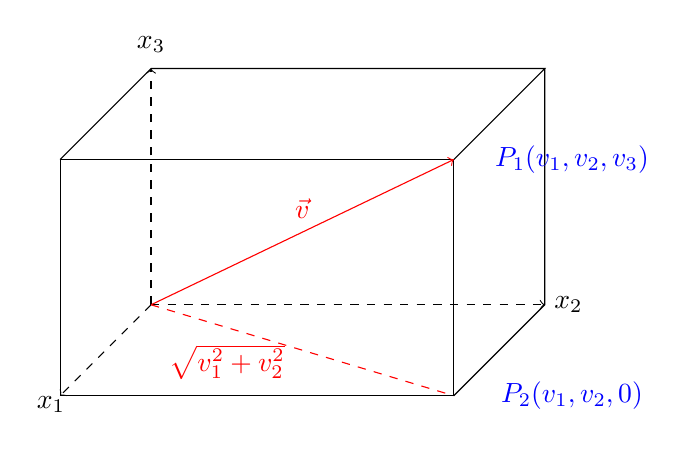
\begin{tikzpicture}
                \draw[dashed, ->] (0,0,0) -- (0,0,3);
                \draw[dashed, ->] (0,0,0) -- (5,0,0);
                \draw[dashed, ->] (0,0,0) -- (0,3,0);
                \draw[dashed, color=red] (0,0,0) -- (5,0,3);
                \draw (0,0,3) -- (5,0,3) -- (5,3,3) -- (0,3,3) -- (0,0,3);
                \draw (0,3,3) -- (0,3,0) -- (5,3,0) -- (5,3,3);
                \draw (5,3,0) -- (5,0,0) -- (5,0,3);
                \draw[->, color=red] (0,0,0) -- (5,3,3);
                \draw (0,0,3.3) node {$x_1$};
                \draw (5.3,0,0) node {$x_2$};
                \draw (0,3.3,0) node {$x_3$};
                \draw (2.5,1.8,1.5) node [color=red]{$\vec{v}$};
                \draw (6.5,3,3) node [color=blue]{$P_1 (v_1, v_2, v_3)$};
                \draw (6.5,0,3) node [color=blue]{$P_2 (v_1, v_2, 0)$};
                \draw (1.7,0,1.9) node [color=red]{$\sqrt{v_1^{2}+v_2^{2}}$};
            \end{tikzpicture}
            \paragraph{} Anhand dieser Graphik lässt sich die Berechnung der Norm eines Vektors $\vec{v}\in\R^3$ verdeutlichen. Für diesen glit: $\text{|}\vec{v}\text{|}=\sqrt{v_1^{2}+v_2^{2}+v_3^{2}}$.
            \paragraph{} Ein Vektor, dessen Norm 1 beträgt wird als normiert oder Einheitsvektor bezeichnet. Für jeden Vektor $\vec{v}\in\R^{3}$ existiert ein Einheitsvektor $\vec{v^{*}}$ , der folgendermaßen definiert wird: $\vec{v^{*}}=\frac{1}{\text{|}\vec{v}\text{|}}*\vec{v}$.

\section{Lineare Abhängigkeit}

    \subsection{Kollinearität und Komplanarität}

\section{Basen und Erzeugendensystem}

    \subsection{Besondere Basen}

        \subsubsection{Orthogonalbasis}

        \subsubsection{Orthonormalbasis}

    \subsection{Basistransformation}

\section{Winkel zwischen Vektoren}\subsection{Orientierte Winkel}

\section{Geraden}
\section{Ebenen}
\section{Skalarprodukt}
